\begin{figure}[t]
    \centering
    \begin{minipage}[t]{0.31\textwidth}
        \centering
        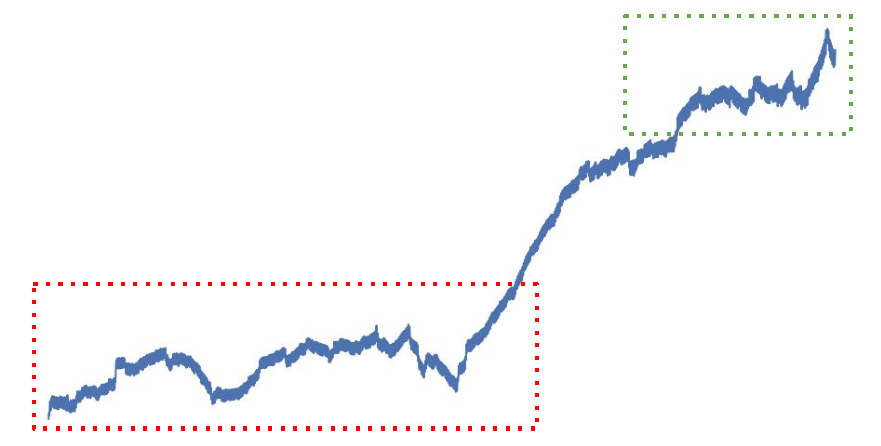
\includegraphics[width=\linewidth]{Images/misc/temporal_shift_traffic.pdf}\\
        (a) Temporal shift.
    \end{minipage}
    \hfill
    \begin{minipage}[t]{0.31\textwidth}
        \centering
        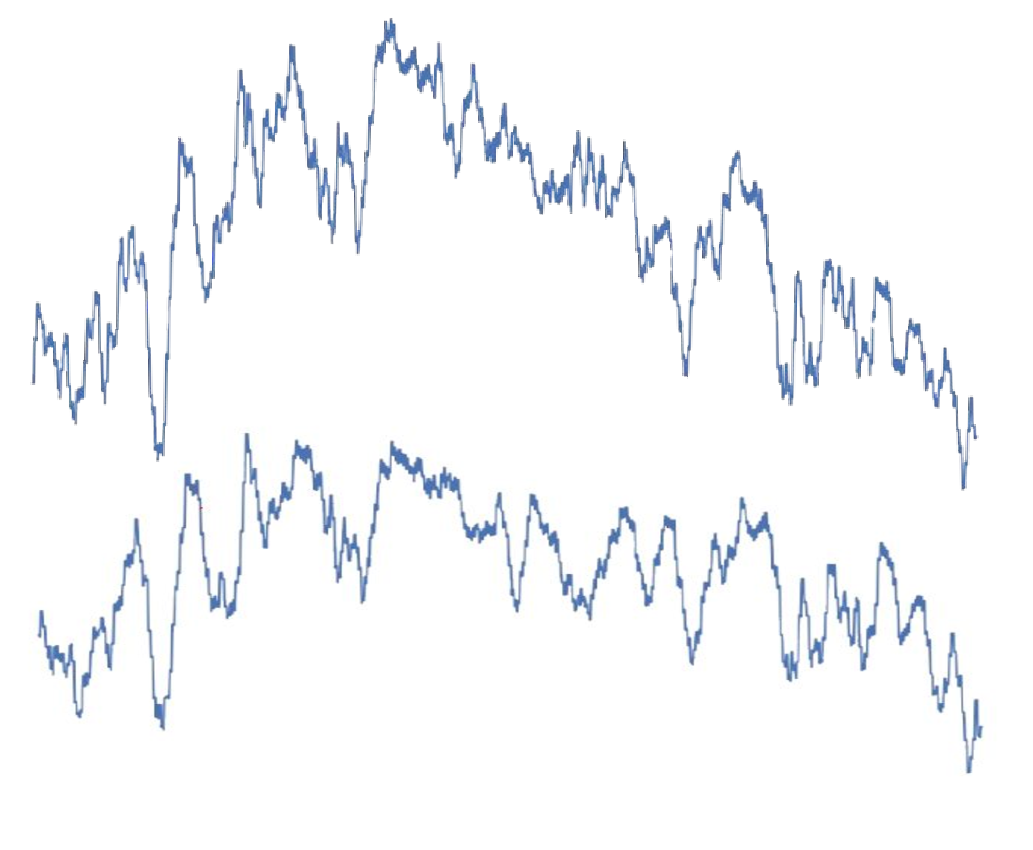
\includegraphics[width=\linewidth]{Images/misc/solar_distrib_shift.pdf}\\
        (b) Spatial shift.
    \end{minipage}
    \hfill
    \begin{minipage}[t]{0.31\textwidth}
        \centering
        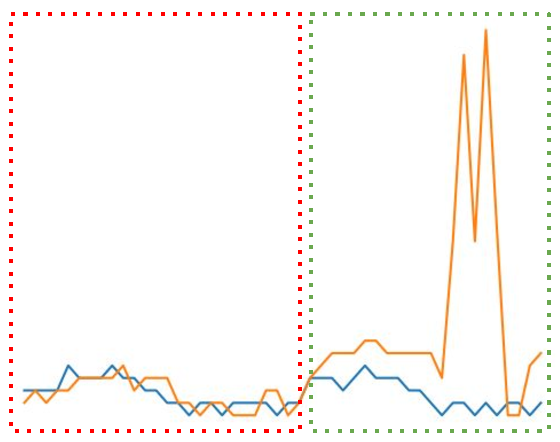
\includegraphics[width=\linewidth]{Images/misc/cond_shift_ecl.pdf}\\
        (c) Conditional shift.
    \end{minipage}
    \caption{Illustration of the three distribution shifts: (a) temporal
    shift between training and test periods (rolling average of a
    \textsc{Traffic} sensor), (b) spatial shift between users (two
    \textsc{Solar} sensors), and (c) conditional shift (different horizons
    for similar look-back windows from one \textsc{Electricity} user).}
    \label{fig:shifts}
\end{figure}
